\documentclass[12pt,a4paper]{article}
\usepackage{amsmath,amssymb}
\usepackage{graphicx}
\usepackage{booktabs}
\usepackage{longtable}
\usepackage{array}
\usepackage{tabularx}
\usepackage{float}
\usepackage{caption}
\usepackage{xcolor}
\usepackage{geometry}
\geometry{a4paper,top=2.2cm,bottom=2.2cm,left=1.8cm,right=1.8cm}
\usepackage{fancyhdr}
\usepackage{enumitem}
\usepackage{titlesec}
\usepackage[hidelinks]{hyperref}
\usepackage{xepersian}

% ---- fonts: B Nazanin for Persian, Times New Roman for Latin ------------
\settextfont[Scale=1.10]{B Nazanin}
\setlatintextfont[Scale=1.00]{Times New Roman}
\setdigitfont[Scale=1.00]{Times New Roman}

% caption setup must come AFTER xepersian: bidi resets it otherwise
\captionsetup{font=small,labelfont=bf,skip=6pt,justification=justified,singlelinecheck=false}
\captionsetup[figure]{position=below}
\captionsetup[table]{position=above}

\linespread{1.35}
\setlength{\parindent}{0pt}
\setlength{\parskip}{5pt}
\titleformat{\section}{\Large\bfseries\color{blue!35!black}}{\thesection}{0.6em}{}
\titleformat{\subsection}{\large\bfseries\color{blue!25!black}}{\thesubsection}{0.5em}{}
\pagestyle{fancy}
\fancyhf{}
\fancyfoot[C]{\thepage}
\fancyhead[R]{\small آزمایشگاه مجازی امواج الکترومغناطیسی}
\renewcommand{\headrulewidth}{0.4pt}
\renewcommand{\figurename}{شکل}
\renewcommand{\tablename}{جدول}
\renewcommand{\contentsname}{فهرست مطالب}
\renewcommand{\listfigurename}{فهرست شکل‌ها}
\DeclareGraphicsExtensions{.png,.pdf,.jpg}
\graphicspath{{../figures/}{figures/}{./}}

\begin{document}

\begin{titlepage}
  \centering
  \vspace*{2.5cm}
  {\Huge\bfseries آزمایشگاه مجازی امواج الکترومغناطیسی\par}
  \vspace{0.6cm}
  {\LARGE\bfseries \lr{EM Virtual Lab}\par}
  \vspace{1.6cm}
  {\Large راهنمای کاربر و توضیح تمام بخش‌های برنامه\par}
  \vspace{0.5cm}
  {\large برخورد موج تخت الکترومغناطیسی با مرز دو محیط\par}
  \vspace{2.2cm}
  {\large درس: میدان‌ها و امواج\par}
  \vspace{0.4cm}
  {\large پیاده‌سازی: \lr{MATLAB} (نسخه \lr{R2021a} یا جدیدتر، بدون جعبه‌ابزار)\par}
  \vspace{2.0cm}
  \begin{tabular}{p{6cm}p{6cm}}
    \hline
    نام دانشجو: & شماره دانشجویی: \\[0.9cm]
    \hline
    تاریخ: & امضا: \\[0.9cm]
    \hline
  \end{tabular}
  \vfill
  {\small نسخۀ سند ۱ \lr{---} آبان ۱۴۰۵\par}
\end{titlepage}

\tableofcontents
\newpage
\listoffigures
\newpage

\section{این برنامه چه می‌کند}

این برنامه یک آزمایشگاه مجازی تعاملی است: موج تخت الکترومغناطیسی به مرز میان دو محیط می‌تابد و برنامه میدان‌های الکتریکی و مغناطیسی، ضرایب بازتاب و عبور، موج ایستا، موج میرا در بازتاب کلی و رفتار رسانای کامل را نشان می‌دهد. همۀ اعداد از روابط درسی محاسبه می‌شوند و در تب «نتایج و تئوری» هم عدد و هم فرمول نمایش داده می‌شود.

قراردادها: محیط ۱ در \lr{z} $<$ 0 و محیط ۲ در \lr{z} $>$ 0؛ صفحۀ برخورد \lr{x-z} و \lr{y} عمود بر آن؛ دامنۀ میدان فرودی $E_0=1$ ولت بر متر؛ وابستگی زمانی به شکل $e^{+j\omega t}$ و بنابراین فازورها به شکل $e^{-j\mathbf{k}\cdot\mathbf{r}}$. برای اینکه محیط ۱ در تصویرها بالا دیده شود، محور \lr{z} معکوس رسم می‌شود.

همۀ خواسته‌های پروژه (\lr{R1} تا \lr{R12)} در برنامه پوشش داده شده‌اند؛ نگاشت هر مورد به محل دقیق آن در برنامه در فایل \lr{\texttt{README.md}} آمده است.

\section{اجرای برنامه و آزمون‌ها}

سه گام اجرا:
\begin{latin}
\begin{verbatim}
cd path\to\EM_VirtualLab
run_lab
\end{verbatim}
\end{latin}

پنجرۀ برنامه با پنج تب باز می‌شود: \lr{Media}، \lr{Field Animation}، \lr{Standing Wave}، \lr{Coefficients vs Angle} و \lr{Results and Theory.} پیشنهاد می‌شود ابتدا در تب \lr{Media} محیط‌ها را تنظیم کنید و بعد به تب‌های دیگر بروید.

آزمون‌های صحت (اختیاری، ولی برای اطمینان از درستی نتایج توصیه می‌شود):
\begin{latin}
\begin{verbatim}
cd tests
test_core        % T1..T12 physics of the core solver
smoke_gui        % 49 GUI checks, headless
fuzz_probe       % sweeps 106 states looking for numerical defects
\end{verbatim}
\end{latin}

نکتۀ مهم: اگر فایل‌های برنامه را تغییر دادید، پنجرۀ باز را ببندید و برنامه را دوباره اجرا کنید؛ متلب نسخۀ قدیمی فایل را در حافظه نگه می‌دارد. برای بستن پنجرۀ گیرکرده در پنجرۀ فرمان متلب بنویسید:
\begin{latin}
\begin{verbatim}
delete(findall(groot,'Type','figure'))
\end{verbatim}
\end{latin}

\section{ساختار پوشه‌ها و فایل‌ها}
\begin{table}[H]
  \centering
  \small
  \caption{ساختار پروژه}
  \begin{tabular}{|p{5.2cm}|p{11.2cm}|}
    \hline
    \textbf{مسیر} & \textbf{توضیح} \\
    \hline
    \lr{\texttt{run\_lab}}.\lr{m} & دستور اجرای برنامه \\
    \hline
    \lr{core/}\lr{\texttt{em\_constants}}.\lr{m} & ثابت‌های فیزیکی (تنها جای تعریف آن‌ها) \\
    \hline
    \lr{core/}\lr{\texttt{em\_defaults}}.\lr{m} & مقادیر پیش‌فرض و تمام اعتبارسنجی ورودی‌ها \\
    \hline
    \lr{core/}\lr{\texttt{em\_solve}}.\lr{m} & اسنل، ضرایب فرنل، بروستر، بحرانی، \lr{PEC} و محیط اتلافی \\
    \hline
    \lr{core/}\lr{\texttt{em\_fields}}.\lr{m} & فازورهای سه موج و میدان کل \\
    \hline
    \lr{core/}\lr{\texttt{em\_standing\_wave}}.\lr{m} & پوش موج ایستا، گره و شکم، \lr{SWR}، جریان و بار سطحی \\
    \hline
    \lr{core/}\lr{\texttt{em\_angle\_sweep}}.\lr{m} & ضرایب برحسب زاویه برای دو قطبش \\
    \hline
    \lr{gui/}\lr{\texttt{EM\_VirtualLab}}.\lr{m} & کل رابط گرافیکی \\
    \hline
    \lr{tests/} & آزمون‌ها، تولید شکل‌ها و اسکرین‌شات‌ها \\
    \hline
    \lr{docs/} & قرارداد، وضعیت، نقشۀ نظری، راهنما، گزارش و همین سند \\
    \hline
    \lr{figures/} & شکل‌ها و تصاویر رابط گرافیکی \\
    \hline
  \end{tabular}
\end{table}

\section{تب \lr{Media} \lr{---} شش ثابت محیط و شش حالت نمونه}

در این تب هر محیط با ثابت‌های الکترومغناطیسی خود تعریف می‌شود. برای هر محیط سه کادر وجود دارد: گذردهی نسبی $\varepsilon_r$، تراوایی نسبی $\mu_r$ و رسانندگی \lr{\texttt{sigma}} برحسب زیمنس بر متر. مقدار $\sigma=0$ یعنی محیط بدون اتلاف.
\begin{table}[H]
  \centering
  \small
  \caption{رنج مجاز ورودی‌ها}
  \begin{tabular}{|p{2.2cm}|p{4.4cm}|p{5.2cm}|p{4.6cm}|}
    \hline
    \textbf{کمیت} & \textbf{معنا} & \textbf{رنج مجاز} & \textbf{پیش‌فرض} \\
    \hline
    $\varepsilon_r$ & گذردهی نسبی & صفر تا $10^{4}$ & محیط ۱: ۱ \lr{---} محیط ۲: ۲.۲۵ \\
    \hline
    $\mu_r$ & تراوایی نسبی & صفر تا $10^{4}$ & ۱ \\
    \hline
    \lr{\texttt{sigma}} & رسانندگی & ۰ تا $10^{9}$ \lr{S/m} & ۰ \\
    \hline
    \lr{f} & بسامد & ۱ مگاهرتز تا ۱۰۰ گیگاهرتز & ۱ گیگاهرتز \\
    \hline
    $\theta_i$ & زاویۀ فرود & ۰ تا ۸۹.۹ درجه & ۰ \\
    \hline
  \end{tabular}
\end{table}

سه کنترل کمکی: منوی «مادۀ آماده» برای پرکردن سریع محیط ۲ (هوا، شیشه، تفلون، آب، \lr{FR-4} با اتلاف، آب دریا و فریت مغناطیسی)؛ دکمۀ «\lr{Swap media}» برای جابه‌جایی دو محیط (راه رسیدن به بازتاب کلی)؛ و منوی «\lr{Simulation mode}» برای انتخاب دی‌الکتریک یا رسانای کامل برای محیط ۲.

کادر گزارش پایین تب، برای هر محیط مقدارهای محاسبه‌شده را نشان می‌دهد: گذردهی مختلط $\varepsilon_c$، ضریب شکست \lr{n}، امپدانس ذاتی $\eta$، طول موج $\lambda$، ثابت تضعیف $\alpha$ و در محیط اتلافی تانژانت اتلاف $\tan\delta$ و عمق پوست $\delta_s$؛ و در پایان نسبت $n_2/n_1$ و $\eta_2/\eta_1$ و زاویۀ بحرانی یا بروستر در صورت وجود. با این کادر می‌توانید فوراً بررسی کنید که ورودی‌ها همان چیزی را می‌دهند که از تئوری انتظار دارید.

\subsection{حالت ۱ \lr{---} هوا به شیشه (دی‌الکتریک بدون اتلاف)}

حالت پیش‌فرض: محیط ۱ هوا و محیط ۲ شیشه با $\varepsilon_r$ = 2.25. ضریب شکست محیط ۲ برابر ۱.۵ و امپدانس آن ۲۵۱.۱۵ اهم می‌شود. زاویۀ بروستر برای قطبش \lr{TM} برابر ۵۶.۳۱ درجه است، ولی زاویۀ بحرانی وجود ندارد چون $n_1$ $<$ $n_2$.
\begin{figure}[H]
  \centering
  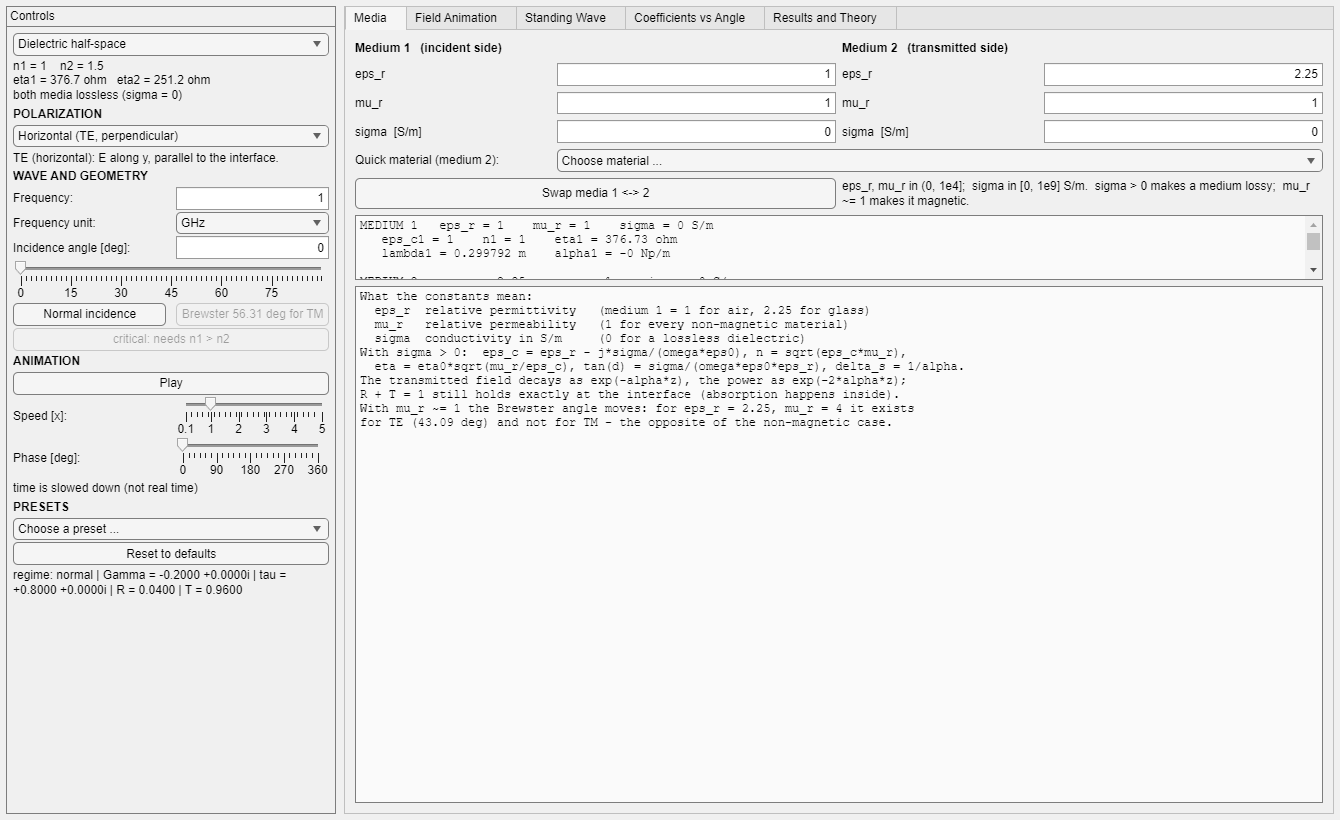
\includegraphics[width=0.98\textwidth]{guide_media_default.png}
  \caption{تب \lr{Media} در حالت هوا به شیشه: شش کادر ثابت‌ها، منوی مادۀ آماده، دکمۀ جابه‌جایی محیط‌ها و کادر گزارش.}
\end{figure}

\subsection{حالت ۲ \lr{---} شیشه به هوا پس از جابه‌جایی: زاویۀ بحرانی ظاهر می‌شود}

با زدن دکمۀ «\lr{Swap media}» مقادیر دو محیط جابه‌جا می‌شوند: محیط ۱ شیشه و محیط ۲ هوا. اکنون $n_1=1.5>n_2=1$ و زاویۀ بحرانی برابر $\arcsin(1/1.5)=41.81$ درجه است؛ دکمۀ «\lr{Go to critical angle}» روشن می‌شود و در کادر گزارش مقدار زاویۀ بحرانی نوشته می‌شود. برای زاویه‌های بزرگ‌تر از $\theta_c$ بازتاب کلی رخ می‌دهد: $|\Gamma|=1$ و $T=0$.
\begin{figure}[H]
  \centering
  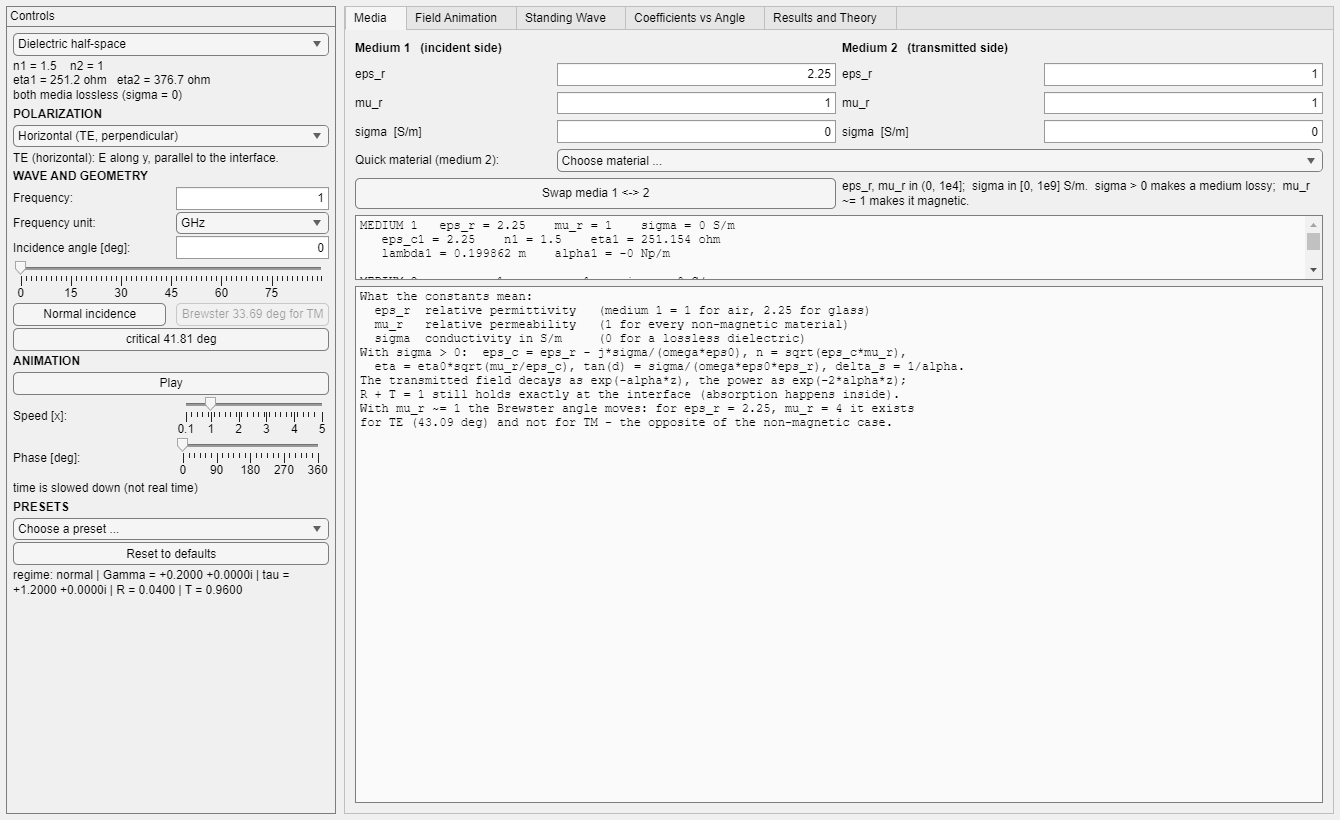
\includegraphics[width=0.98\textwidth]{guide_media_tir.png}
  \caption{همان تب پس از جابه‌جایی محیط‌ها: $n_1=1$.5 و $n_2=1$ و زاویۀ بحرانی ۴۱.۸۱ درجه.}
\end{figure}

\subsection{حالت ۳ \lr{---} محیط ۲ با اتلاف (\lr{FR-4} با $\sigma=0$.02 \lr{S/m)}}

با مثبت‌شدن رسانندگی، محیط اتلافی می‌شود و برنامه با گذردهی مختلط کار می‌کند: $\varepsilon_c=\varepsilon_r-j\sigma/(\omega\varepsilon_0)$. برای \lr{FR-4} در ۱ گیگاهرتز: $\mathrm{Re}(\varepsilon_c)=4.4$، $-\mathrm{Im}(\varepsilon_c)=0.3595$، تانژانت اتلاف 0.0817، ثابت تضعیف $\alpha=1.7945$ بر متر و عمق پوست $\delta_s=0.5573$ متر. موج عبوری به‌صورت $e^{-\alpha z}$ میرا می‌شود و توان آن با $e^{-2\alpha z}$ کاهش می‌یابد. در مرز همچنان $R+T=1$ برقرار است، چون اتلاف درون محیط رخ می‌دهد نه روی مرز. محیط اتلافی بازتاب کلی واقعی و زاویۀ بروستر دقیق ندارد (برنامه «\lr{none}» گزارش می‌کند).
\begin{figure}[H]
  \centering
  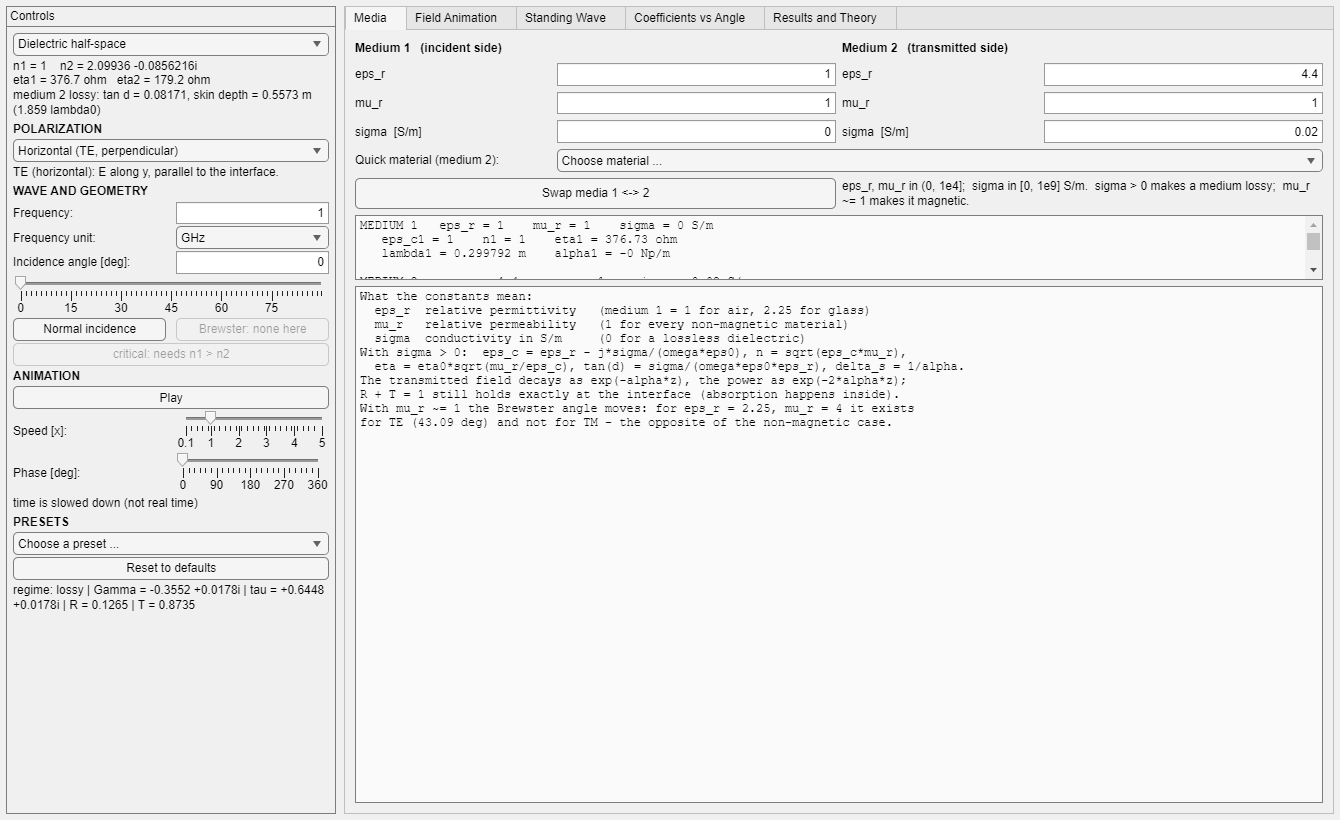
\includegraphics[width=0.98\textwidth]{guide_media_lossy.png}
  \caption{تب \lr{Media} برای \lr{FR-4} با اتلاف: تانژانت اتلاف و عمق پوست در کادر گزارش دیده می‌شود و گذردهی و ضریب شکست به‌صورت مختلط نمایش داده می‌شوند.}
\end{figure}

\subsection{حالت ۴ \lr{---} اتلاف شدید: آب دریا با \lr{\texttt{sigma}} = 4 \lr{S/m}}

آب دریا با $\varepsilon_r$ = 81 و $\sigma$ = 4 \lr{S/m} نمونۀ یک محیط بسیار اتلافی است: تانژانت اتلاف حدود ۰.۸۹ و عمق پوست چند سانتی‌متر می‌شود، یعنی موج عملاً در لایۀ نازکی نزدیک سطح جذب می‌شود. این حالت تفاوت «محیط اتلافی» و «بازتاب کلی» را روشن می‌کند: در بازتاب کلی هیچ توانی وارد محیط ۲ نمی‌شود، ولی در محیط اتلافی توان وارد می‌شود و درون آن جذب می‌گردد.
\begin{figure}[H]
  \centering
  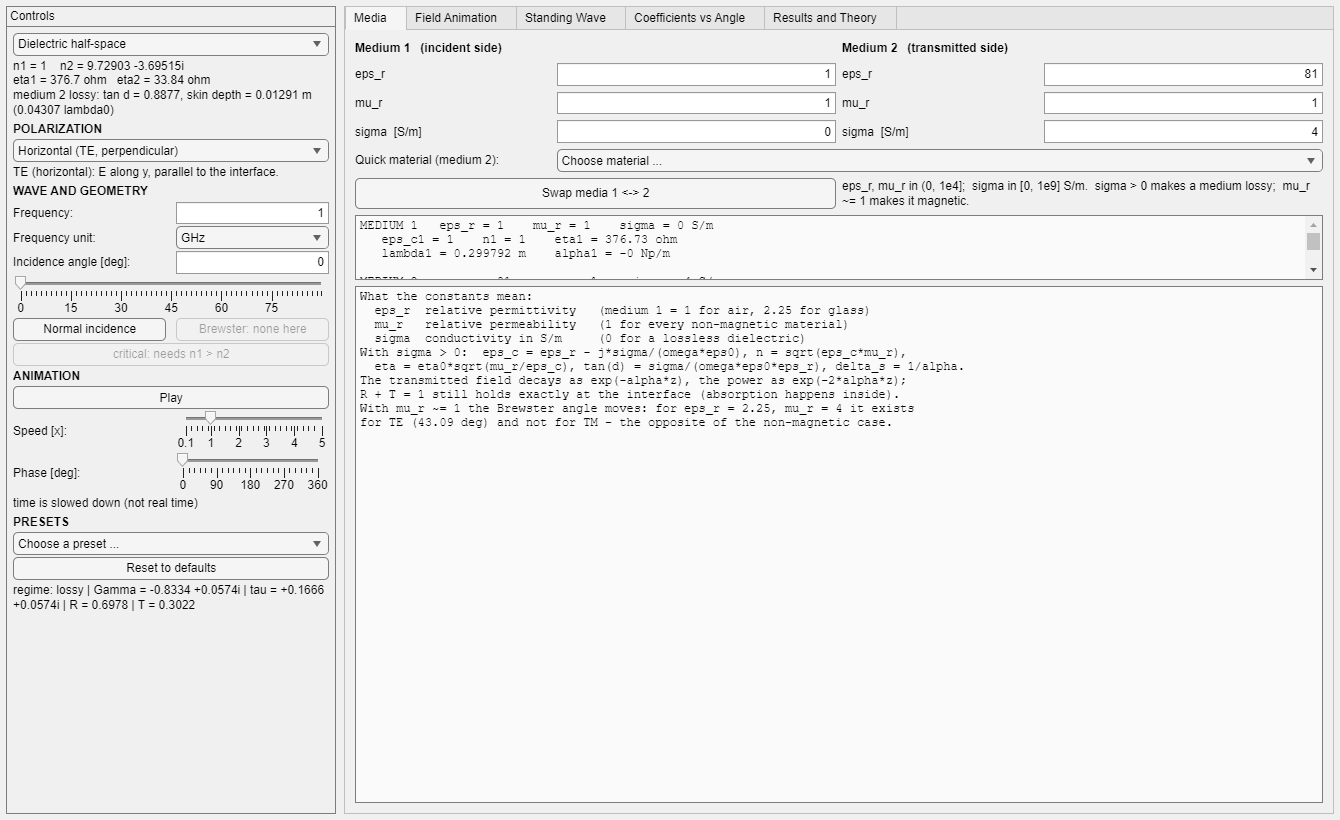
\includegraphics[width=0.98\textwidth]{guide_media_sea.png}
  \caption{آب دریا در ۱ گیگاهرتز: تانژانت اتلاف بزرگ و عمق پوست کوچک.}
\end{figure}

\subsection{حالت ۵ \lr{---} محیط مغناطیسی با $\mu_r$ = 4: بروستر به قطبش \lr{TE} می‌رود}

با بزرگ‌تر شدن تراوایی نسبی محیط ۲، روابط \lr{n} = $\sqrt{\varepsilon_r\mu_r}$ و $\eta$ = $\eta_0\sqrt{\mu_r/\varepsilon_r}$ تغییر می‌کنند و جای زاویۀ بروستر عوض می‌شود. برای $\varepsilon_r$ = 2.25 و $\mu_r$ = 4: $n_2=3$ و $\eta_2=502.3$ اهم. در این حالت زاویۀ بروستر برای قطبش \lr{TE} در ۴۳.۰۹ درجه وجود دارد و برای \lr{TM} وجود ندارد \lr{---} برعکس حالت غیرمغناطیسی که فقط \lr{TM} زاویۀ بروستر دارد. برچسب دکمۀ بروستر همین وضعیت را نشان می‌دهد.
\begin{figure}[H]
  \centering
  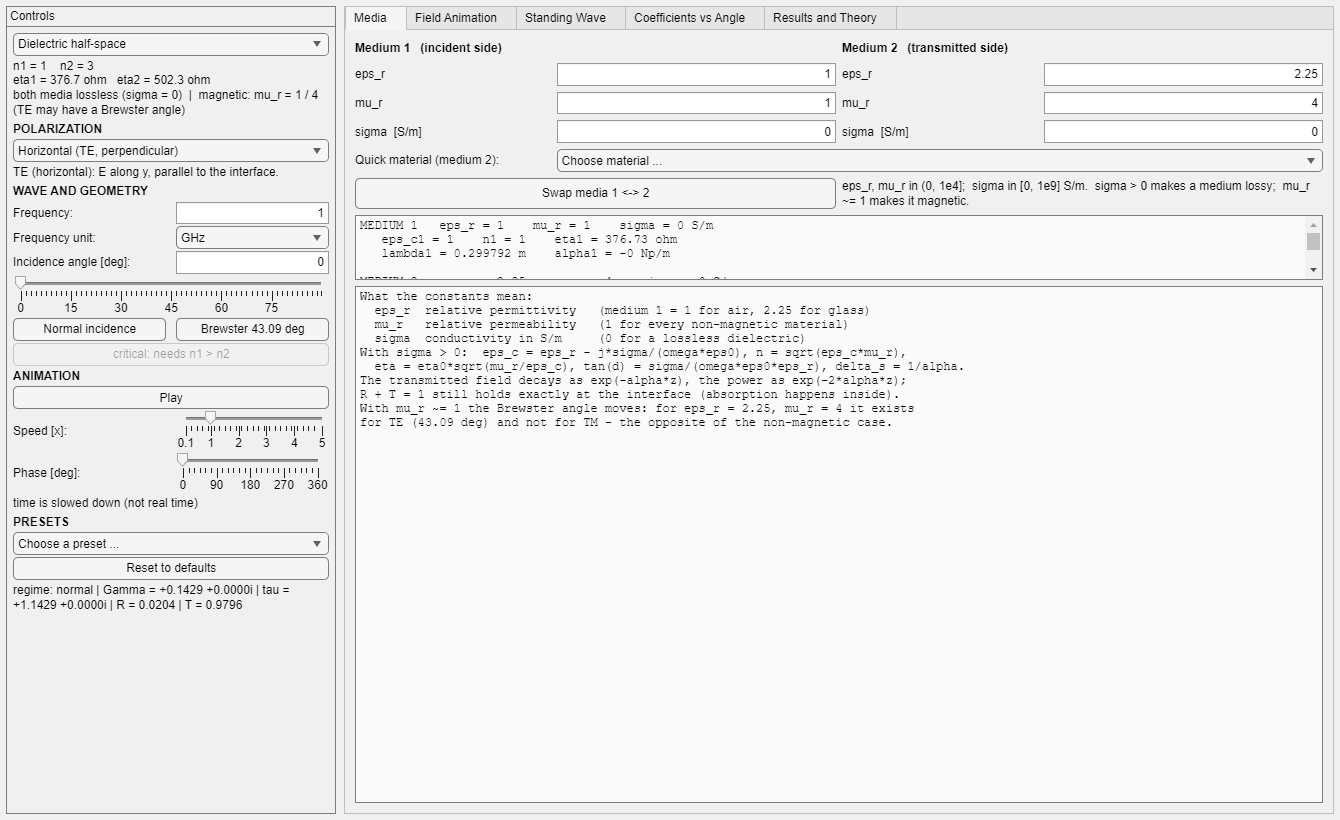
\includegraphics[width=0.98\textwidth]{guide_media_magnetic.png}
  \caption{محیط ۲ مغناطیسی با $\mu_r$ = 4: $n_2=3$ و $\eta_2=502.3$ اهم و یادآوری زاویۀ بروستر قطبش \lr{TE.}}
\end{figure}
\begin{table}[H]
  \centering
  \small
  \caption{فرمول‌های کلیدی محیط}
  \begin{tabular}{|p{6.2cm}|p{10.2cm}|}
    \hline
    \textbf{کمیت} & \textbf{رابطه} \\
    \hline
    ضریب شکست & \lr{n} = $\sqrt{\varepsilon_r\mu_r}$ \\
    \hline
    امپدانس ذاتی & $\eta$ = $\eta_0$ $\surd$($\mu_r$/$\varepsilon_r$) \\
    \hline
    گذردهی مختلط & $\varepsilon_c=\varepsilon_r-j\sigma/(\omega\varepsilon_0)$ \\
    \hline
    تانژانت اتلاف & $\tan\delta=\sigma/(\omega\varepsilon_0\varepsilon_r)$ \\
    \hline
    ثابت تضعیف و عمق پوست & $\alpha=-\mathrm{Im}(k_z),\quad \delta_s=1/\alpha$ \\
    \hline
    میرایی میدان و توان & $|E|\propto e^{-\alpha z},\quad P\propto e^{-2\alpha z}$ \\
    \hline
  \end{tabular}
\end{table}

\subsection{حالت ۶ \lr{---} رسانای کامل (\lr{PEC)}}

با انتخاب «\lr{Perfect conductor} (\lr{PEC)}» از منوی \lr{Simulation mode}، محیط ۲ رسانای کامل می‌شود: کادرهای محیط ۲ غیرفعال می‌شوند، $\Gamma=-1$ و $\tau$ = ۰، میدان در \lr{z} $>$ 0 صفر است و پوش میدان الکتریکی در محیط ۱ به شکل $2|\sin(k_{z1}z)|$ با گره روی سطح ظاهر می‌شود. برنامه جریان سطحی $|J_s|=2|H_i|\cos\theta_i$ برای \lr{TE} یا $|J_s|=2|H_i|$ برای \lr{TM} و بار سطحی $\rho_s=2\varepsilon_0\varepsilon_r\sin\theta_i$ در قطبش \lr{TM} را نیز گزارش می‌کند.
\begin{figure}[H]
  \centering
  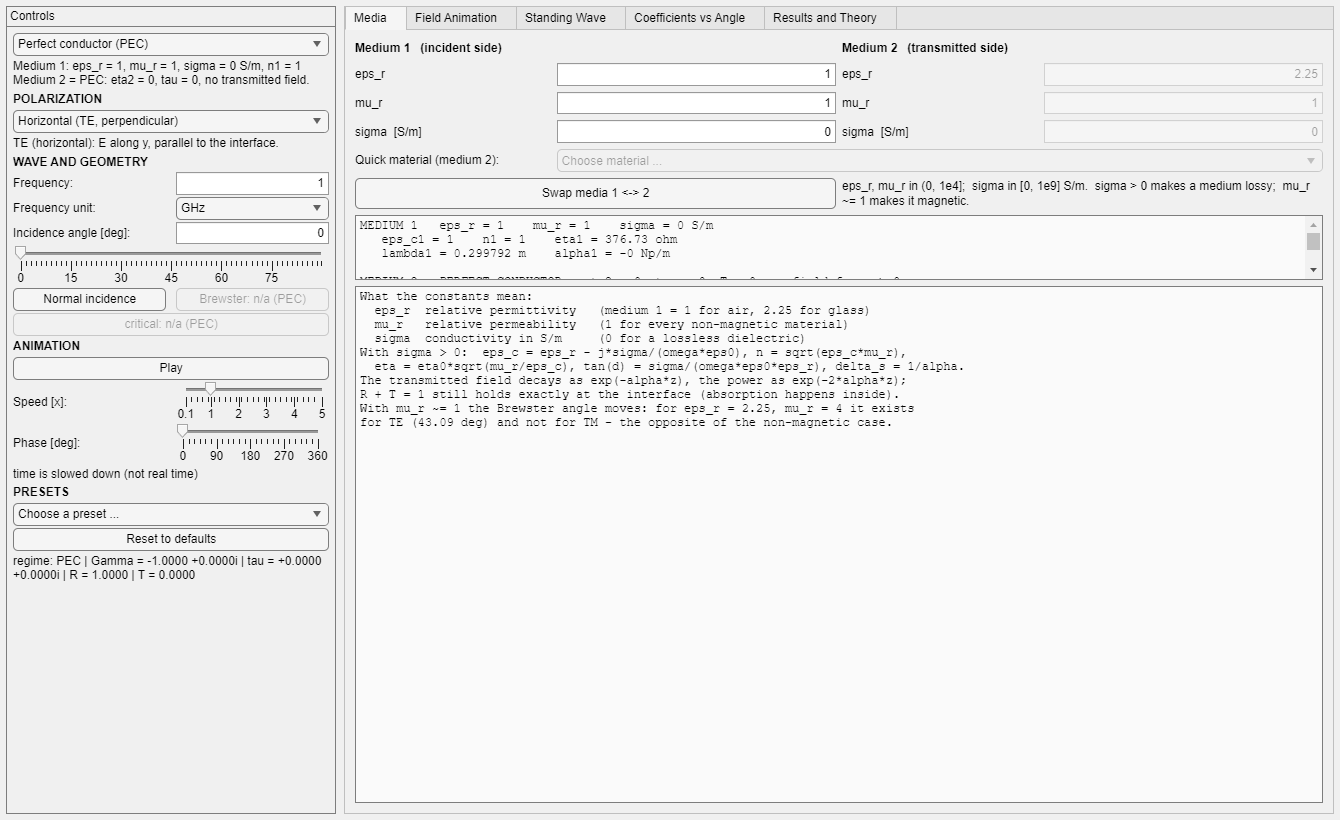
\includegraphics[width=0.98\textwidth]{guide_media_pec.png}
  \caption{حالت \lr{PEC:} کادرهای محیط ۲ غیرفعال و میدان عبوری صفر است.}
\end{figure}

\section{تب \lr{Field Animation} \lr{---} نقشه‌های میدان و انیمیشن}

در این تب دو نقشۀ رنگی کنار هم رسم می‌شود: میدان الکتریکی در چپ و میدان مغناطیسی در راست. محور \lr{z} معکوس است تا محیط ۱ بالا و محیط ۲ پایین دیده شود. مرز \lr{z} = 0 با خط مشکی و نرمال با خط‌چین نشان داده می‌شود و نام هر محیط روی تصویر نوشته شده است.

نوار ابزار بالای تب سه چک‌باکس \lr{Incident} و \lr{Reflected} و \lr{Transmitted} دارد (اگر هر سه تیک داشته باشند میدان کل رسم می‌شود)، گزینۀ افزودن بردارهای میدان، منوهای انتخاب مؤلفۀ رسم‌شده در هر نقشه و کادر اندازۀ پنجرۀ نمایش برحسب طول موج فضای آزاد.

بالای نقشه‌ها یک بلوک متنی جهت‌های انتشار و زاویه‌ها را گزارش می‌کند (در \lr{PEC} عبارت «\lr{no transmitted wave}» و در بازتاب کلی «\lr{evanescent}» همراه با $\alpha$ و $\delta$) و زیر نقشه‌ها نوار وضعیت سه‌خطی است: فاز و بسامد و طول موج و رژیم؛ سپس $\theta_i$ و $\theta_r$ و $\theta_t$؛ و در خط سوم بیشینۀ همان مؤلفه‌هایی که رسم شده‌اند.
\begin{figure}[H]
  \centering
  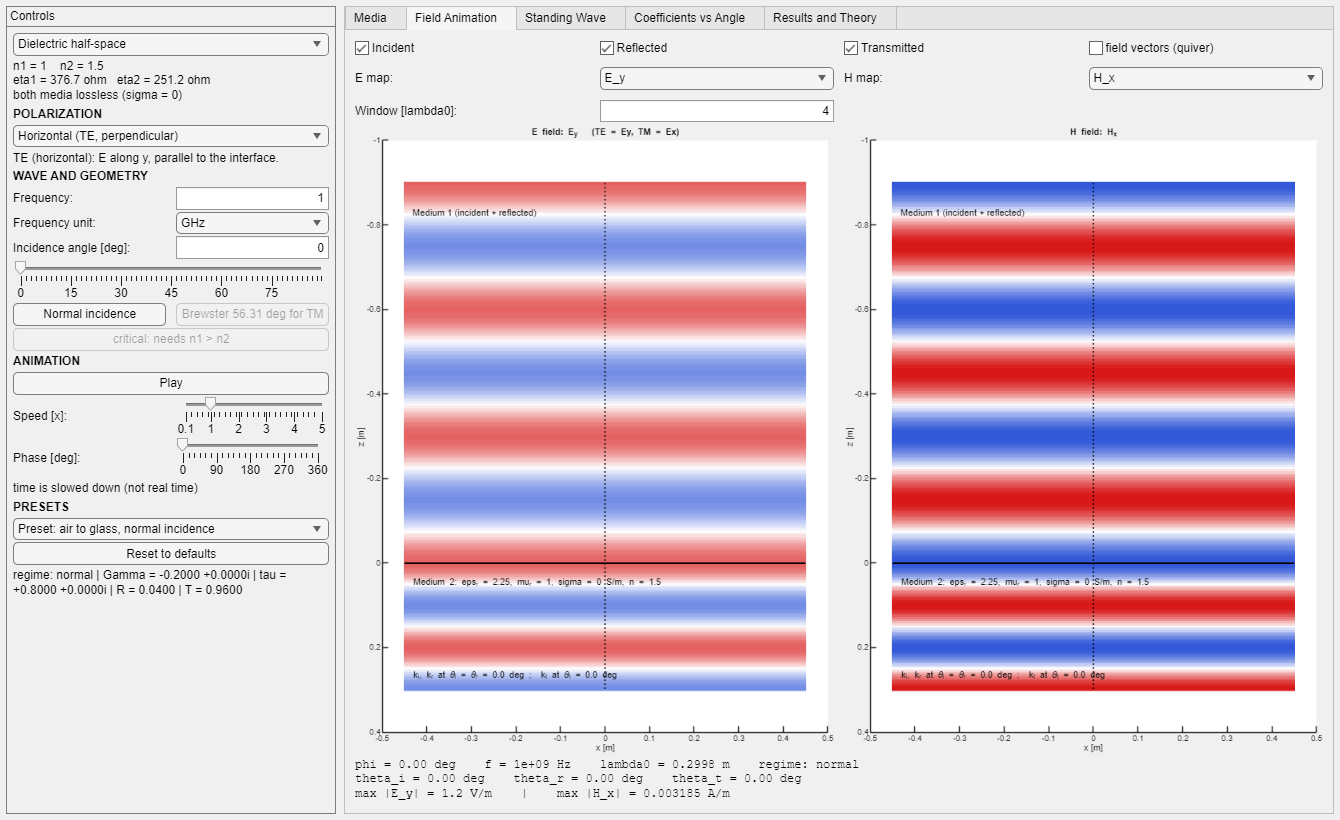
\includegraphics[width=0.98\textwidth]{fig6_gui_fields_dielectric.png}
  \caption{تب \lr{Field Animation} در حالت هوا به شیشه با فرود عمودی و قطبش \lr{TE}؛ مؤلفه‌های \lr{E\_y} و \lr{H\_x} رسم شده‌اند.}
\end{figure}
\begin{figure}[H]
  \centering
  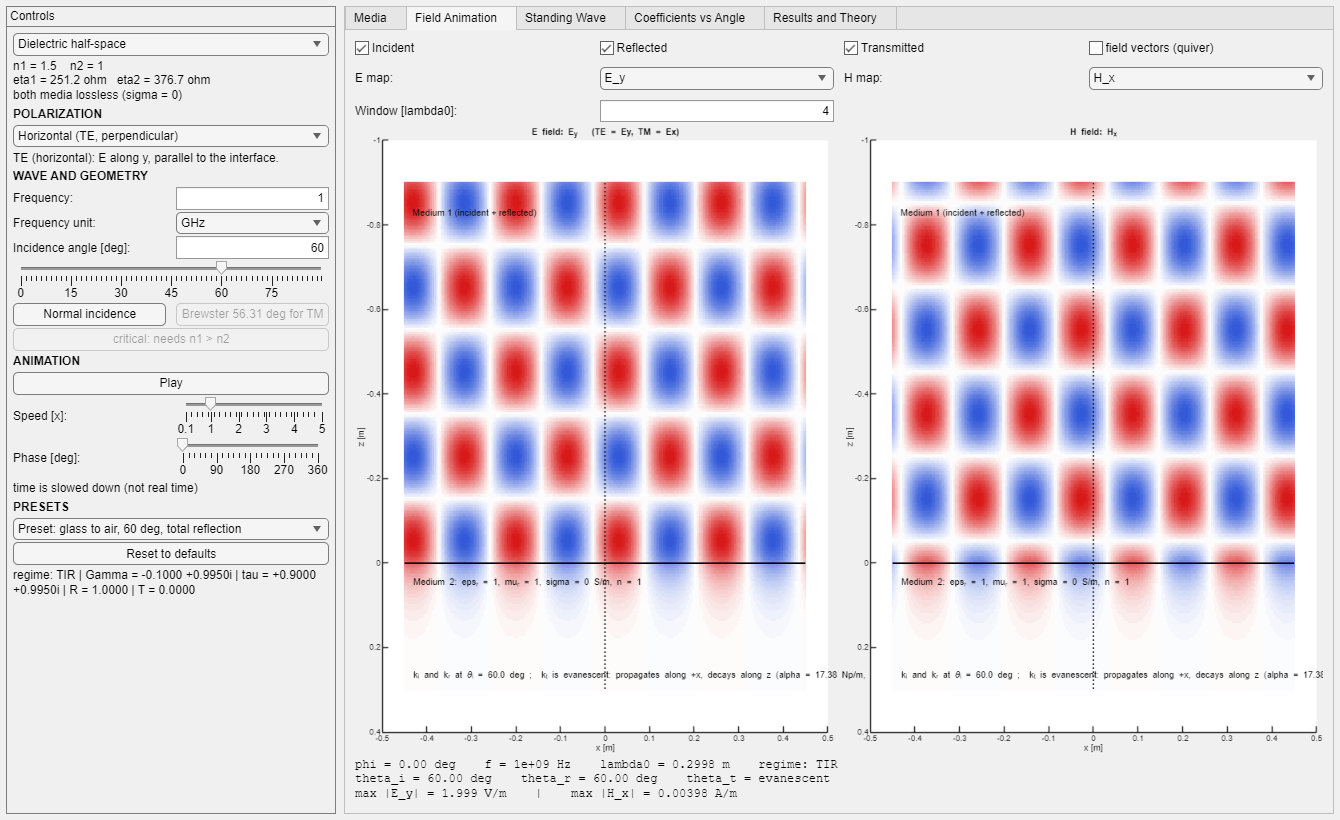
\includegraphics[width=0.98\textwidth]{fig6_gui_fields_tir.png}
  \caption{بازتاب کلی (شیشه به هوا، ۶۰ درجه): میدان میرا در محیط ۲ و گزارش $\alpha$ و $\delta$ در بلوک متن.}
\end{figure}
\begin{figure}[H]
  \centering
  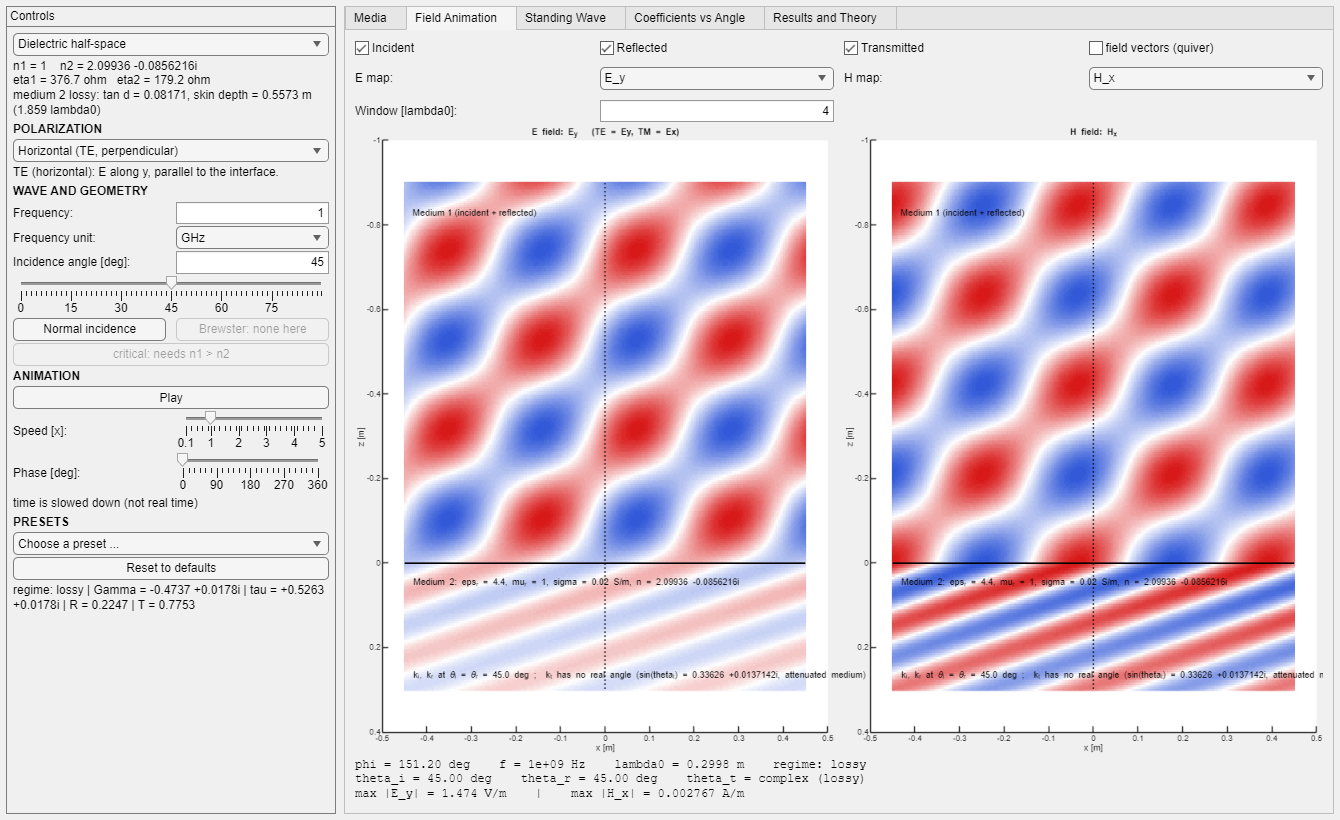
\includegraphics[width=0.98\textwidth]{guide_field_lossy.png}
  \caption{محیط ۲ اتلافی (\lr{FR-4):} موج عبوری به‌سرعت میرا می‌شود و برچسب محیط ۲ مقدارهای $\varepsilon_r$ و $\mu_r$ و \lr{\texttt{sigma}} و ضریب شکست مختلط را نشان می‌دهد.}
\end{figure}
\begin{figure}[H]
  \centering
  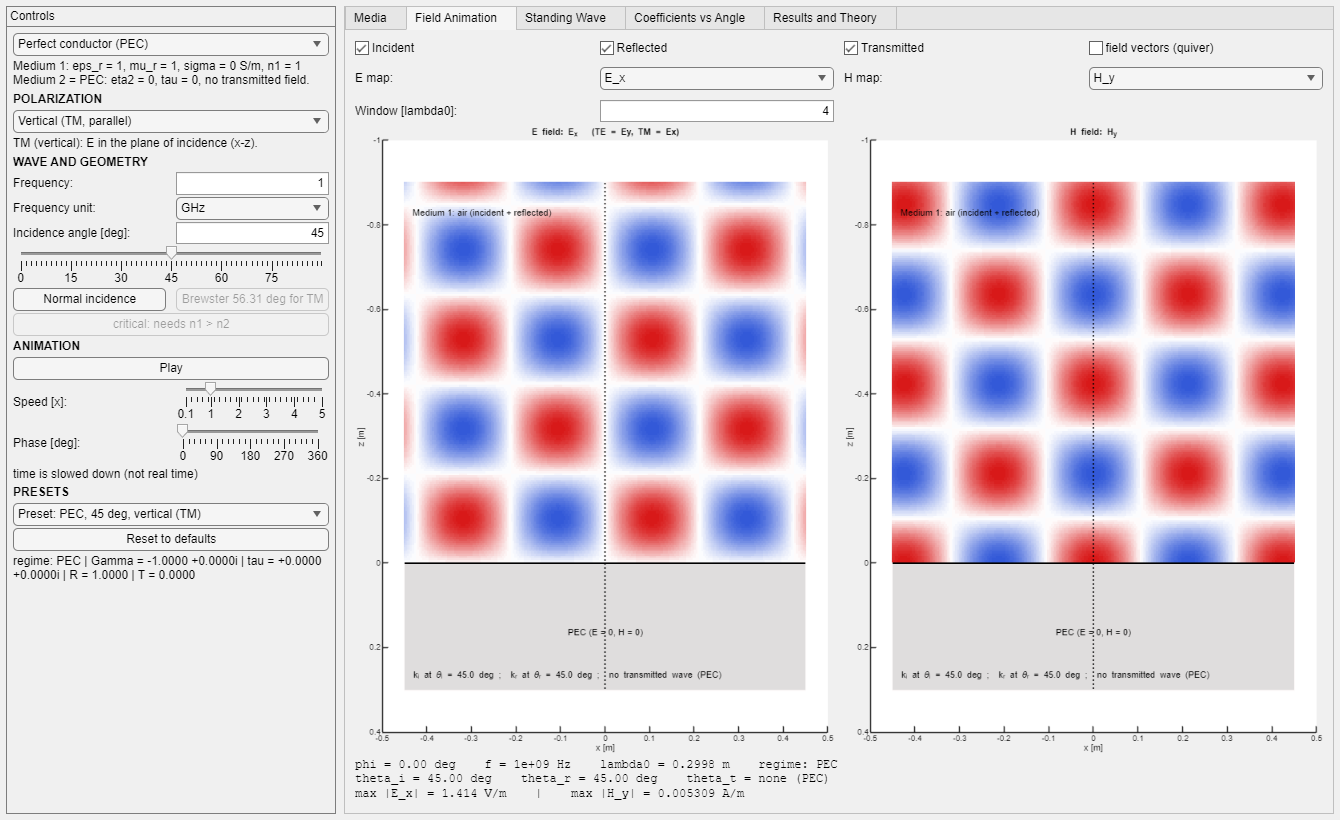
\includegraphics[width=0.98\textwidth]{fig6_gui_fields_pec_tm.png}
  \caption{\lr{PEC} با قطبش \lr{TM:} مؤلفه‌های غالب \lr{E\_x} و \lr{H\_y} هستند و نوار وضعیت بیشینۀ همان دو مؤلفه را گزارش می‌کند.}
\end{figure}

\section{تب \lr{Standing Wave} \lr{---} موج ایستا، گره و شکم}

دو محور، پوش میدان (خط پر مشکی) و مقدار لحظه‌ای (خط آبی) را برحسب \lr{z} نشان می‌دهند؛ خط نقطه‌چین مرز، دایرۀ قرمز گره‌ها و مربع سبز شکم‌ها هستند. پوش، اندازۀ فازور میدان است و در محیط ۱ بدون اتلاف دقیقاً همان رابطۀ کتاب $|1\pm\Gamma e^{2jk_{z1}z}|$ می‌شود. خط آبی مقدار واقعی میدان در لحظۀ جاری است و همیشه داخل پوش می‌ماند.
\begin{itemize}[rightmargin=1.2em,itemsep=2pt,topsep=3pt,label={$\bullet$}]
  \item در محیط ۱ موج ایستای جزئی دیده می‌شود و نسبت موج ایستا $\mathrm{SWR}=\frac{1+|\Gamma|}{1-|\Gamma|}$ گزارش می‌شود.
  \item در محیط ۲ موج عبوری رسم می‌شود: پوش ثابت برای محیط بدون اتلاف و کاهش نمایی در بازتاب کلی یا محیط اتلافی.
  \item جدول زیر نمودارها مکان چند گره و شکم اول را برحسب متر و برحسب $\lambda_1$ می‌دهد.
  \item در حالت \lr{PEC} گره‌های میدان الکتریکی روی سطح و در فاصله‌های $\lambda_1/2$ قرار دارند و \lr{SWR} بی‌نهایت می‌شود.
  \item اگر محیط ۱ اتلافی باشد موج ایستای متناوب تشکیل نمی‌شود و \lr{SWR} تعریف‌نشده گزارش می‌شود.
\end{itemize}
\begin{figure}[H]
  \centering
  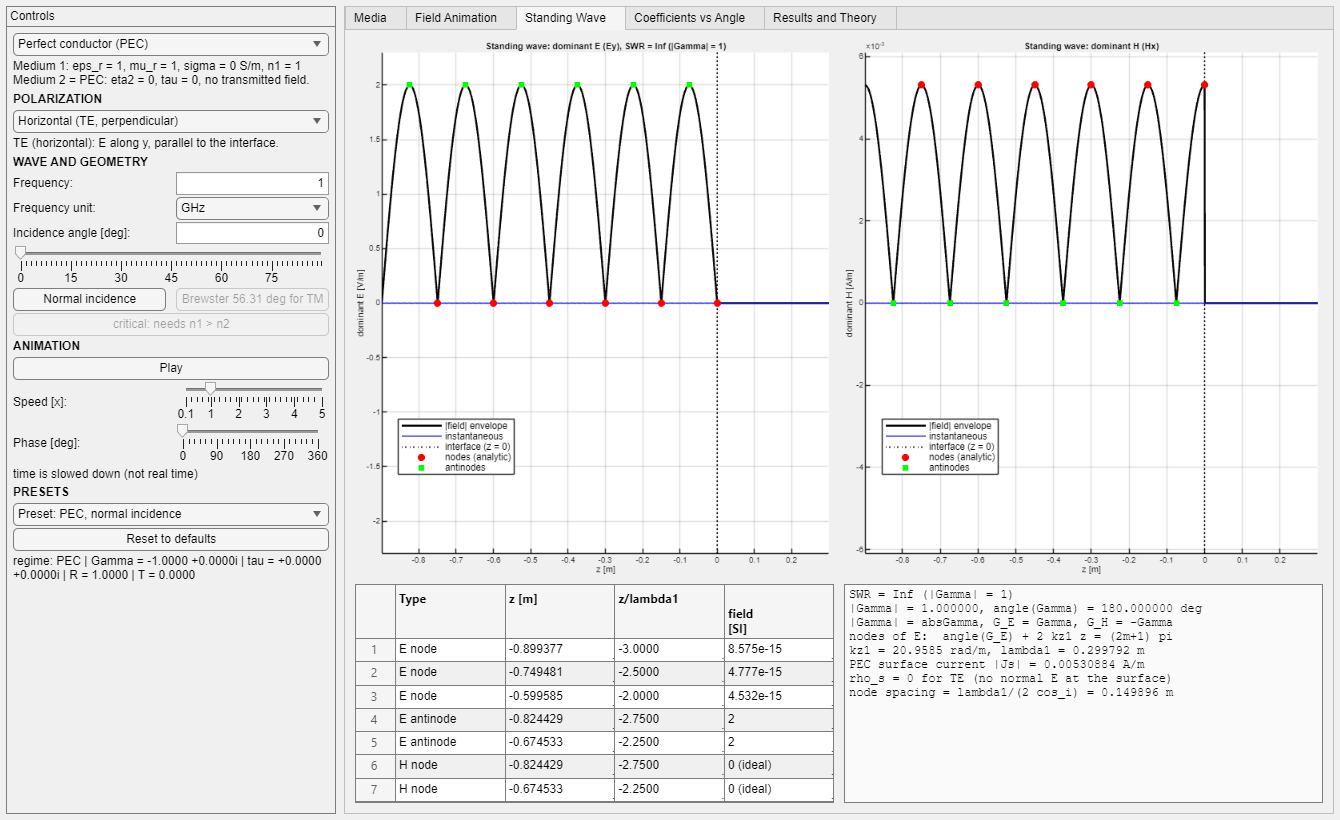
\includegraphics[width=0.98\textwidth]{fig6_gui_standing_pec.png}
  \caption{حالت \lr{PEC:} پوش $2|\sin(k_{z1}z)|$، گره‌ها روی سطح و در فاصله‌های $\lambda_1/2$، \lr{SWR} بی‌نهایت و گزارش جریان سطحی.}
\end{figure}
\begin{figure}[H]
  \centering
  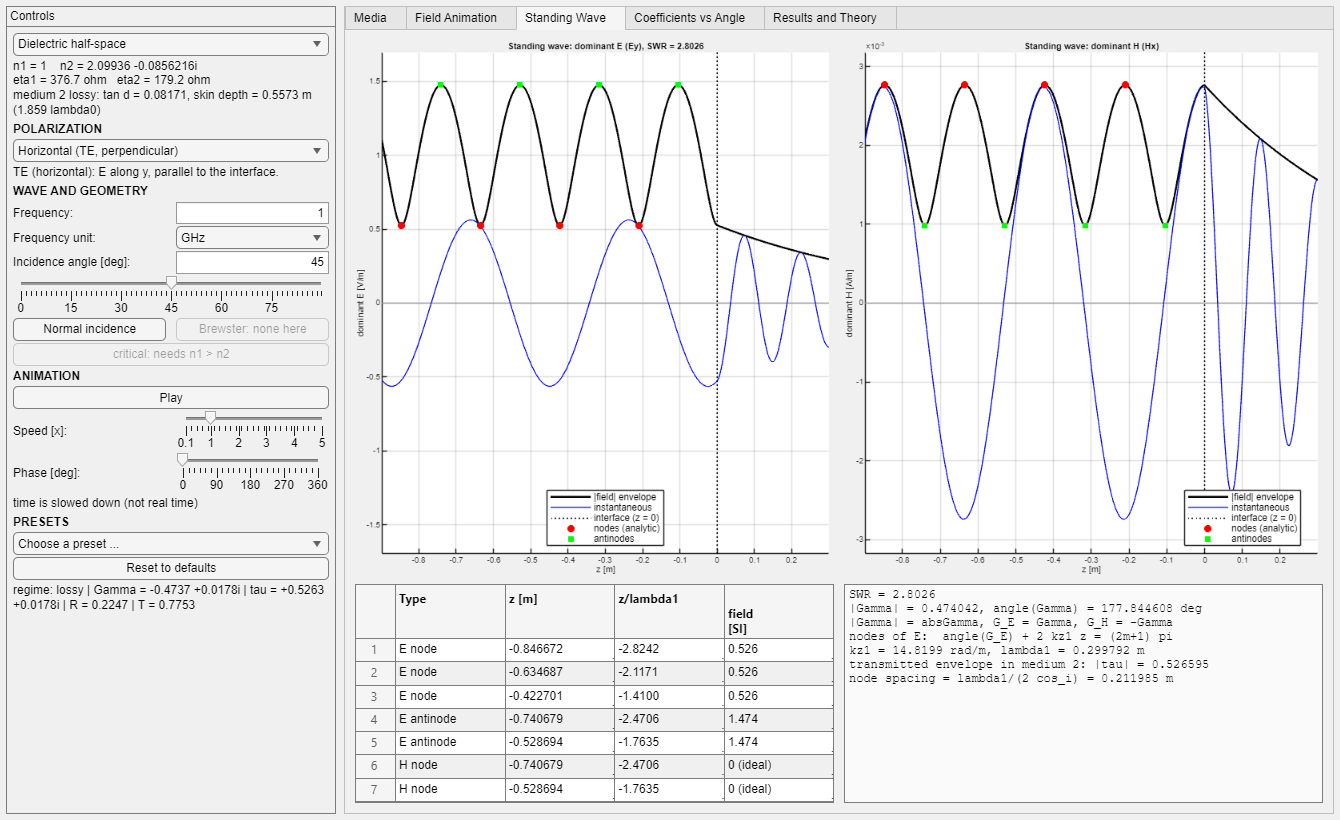
\includegraphics[width=0.98\textwidth]{guide_standing_lossy.png}
  \caption{محیط ۲ اتلافی: پوش درون محیط ۲ کاهش نمایی دارد و عمق پوست گزارش می‌شود.}
\end{figure}

\section{تب \lr{Coefficients vs Angle} \lr{---} ضرایب برحسب زاویه}

چهار نمودار، اندازۀ $\Gamma$، فاز $\Gamma$، اندازۀ $\tau$ و فاز $\tau$ را برحسب زاویۀ فرود از ۰ تا ۸۹.۹ درجه نشان می‌دهند؛ قطبش \lr{TE} با خط پر و \lr{TM} با خط‌چین و قطبش انتخاب‌شده ضخیم‌تر است. خط عمودی سبز زاویۀ بروستر و خط بنفش زاویۀ بحرانی را علامت می‌زند و خط مشکی زاویۀ جاری را نشان می‌دهد. با منوی بالای تب می‌توان به‌جای دامنه، توان‌های \lr{R} و \lr{T} را دید. در جایی که دامنه صفر است خط فاز شکسته می‌شود چون فاز در آن نقطه تعریف نشده است.
\begin{figure}[H]
  \centering
  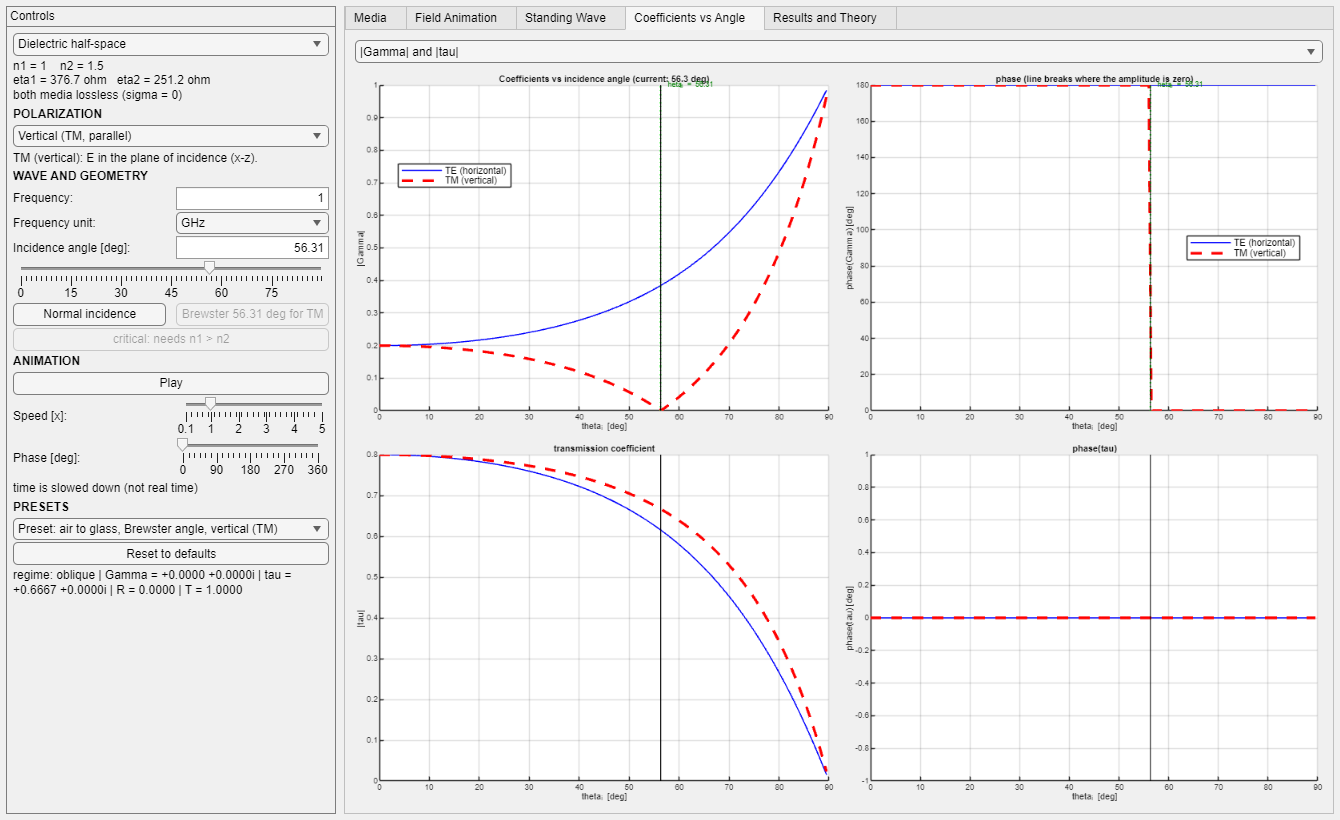
\includegraphics[width=0.98\textwidth]{fig6_gui_coefficients_brewster_tm.png}
  \caption{قطبش \lr{TM:} در زاویۀ بروستر ۵۶.۳۱ درجه اندازۀ $\Gamma$ به صفر می‌رسد.}
\end{figure}
\begin{figure}[H]
  \centering
  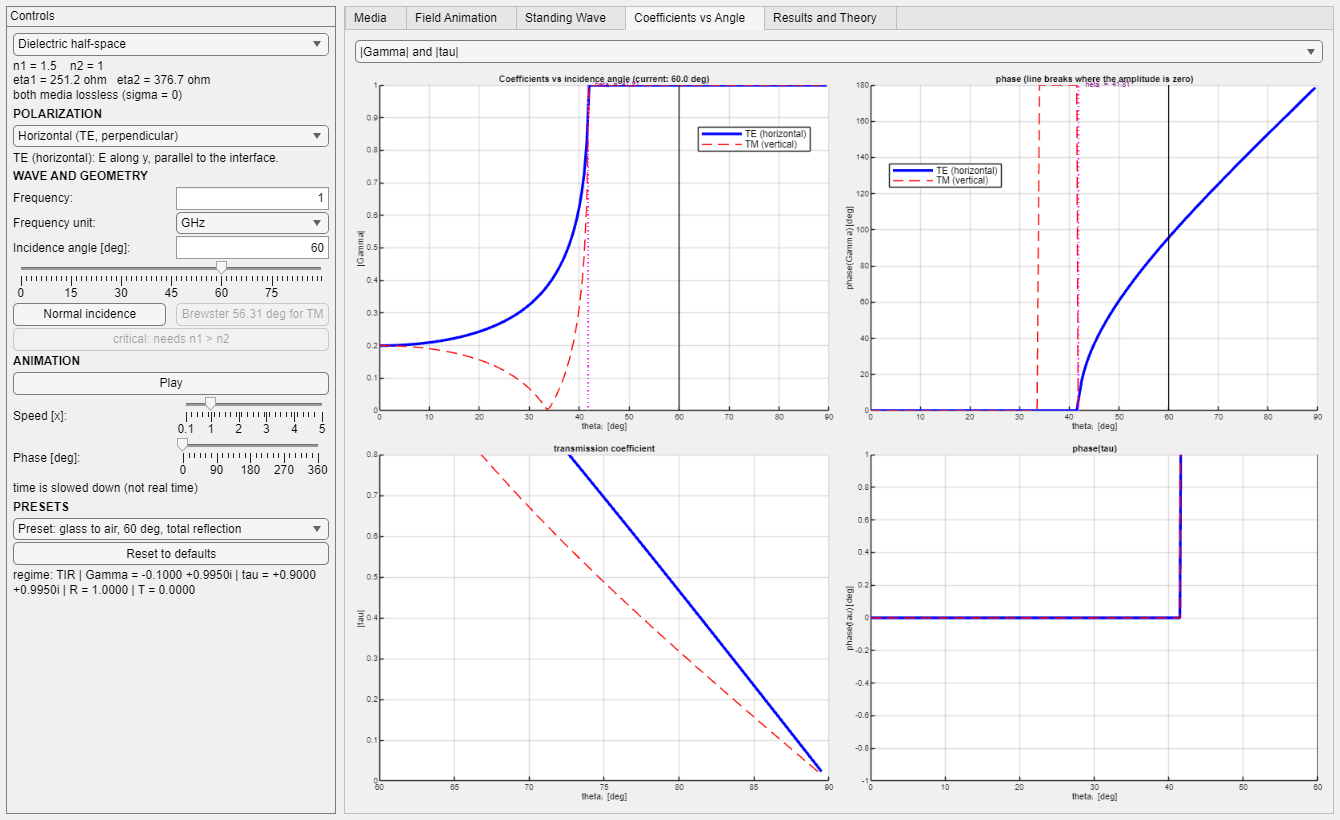
\includegraphics[width=0.98\textwidth]{fig6_gui_coefficients_tir.png}
  \caption{شیشه به هوا: پس از زاویۀ بحرانی ۴۱.۸۱ درجه اندازۀ $\Gamma$ برای هر دو قطبش به ۱ می‌رسد و \lr{T} صفر می‌شود.}
\end{figure}
\begin{figure}[H]
  \centering
  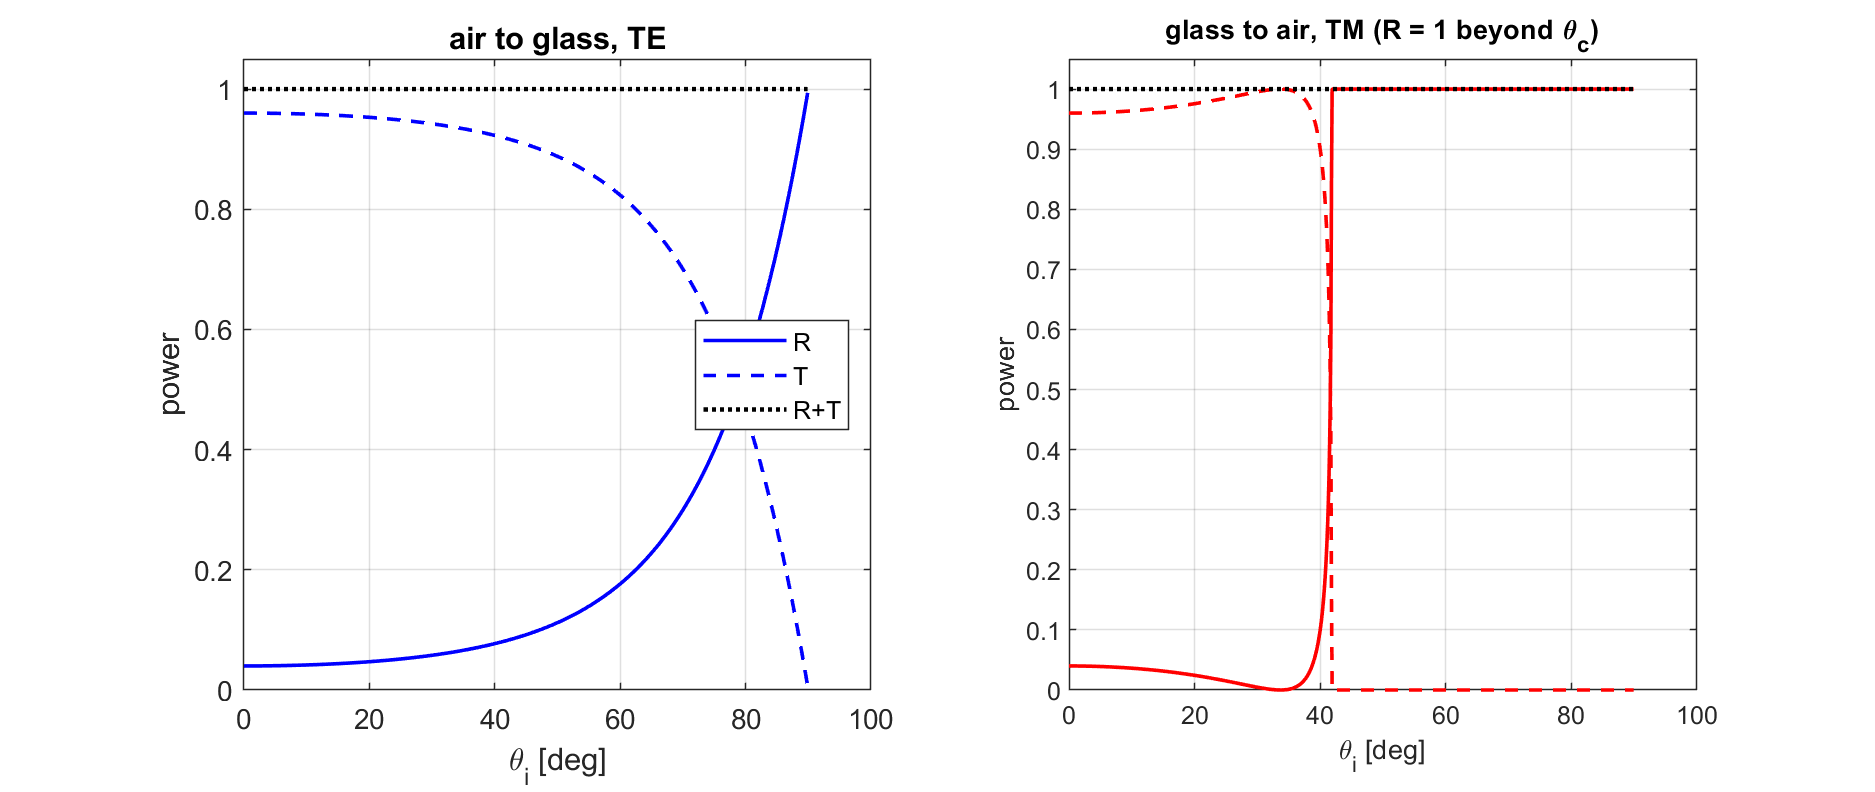
\includegraphics[width=0.98\textwidth]{fig3_power_balance.png}
  \caption{تأیید $R+T=1$ در هر دو جهت انتشار.}
\end{figure}

\section{تب \lr{Results and Theory} \lr{---} نتایج عددی و روابط}

ستون چپ پنل متنی مونواسپیس با بلوک‌های پارامترها، محیط‌ها، هندسه، ضرایب، نتایج موج ایستا و پارامترهای محاسباتی است. ستون راست همان روابط را به‌صورت فرمول نمایش می‌دهد تا هنگام ارائۀ شفاهی بتوانید هر عدد را به رابطۀ آن نسبت دهید.
\begin{figure}[H]
  \centering
  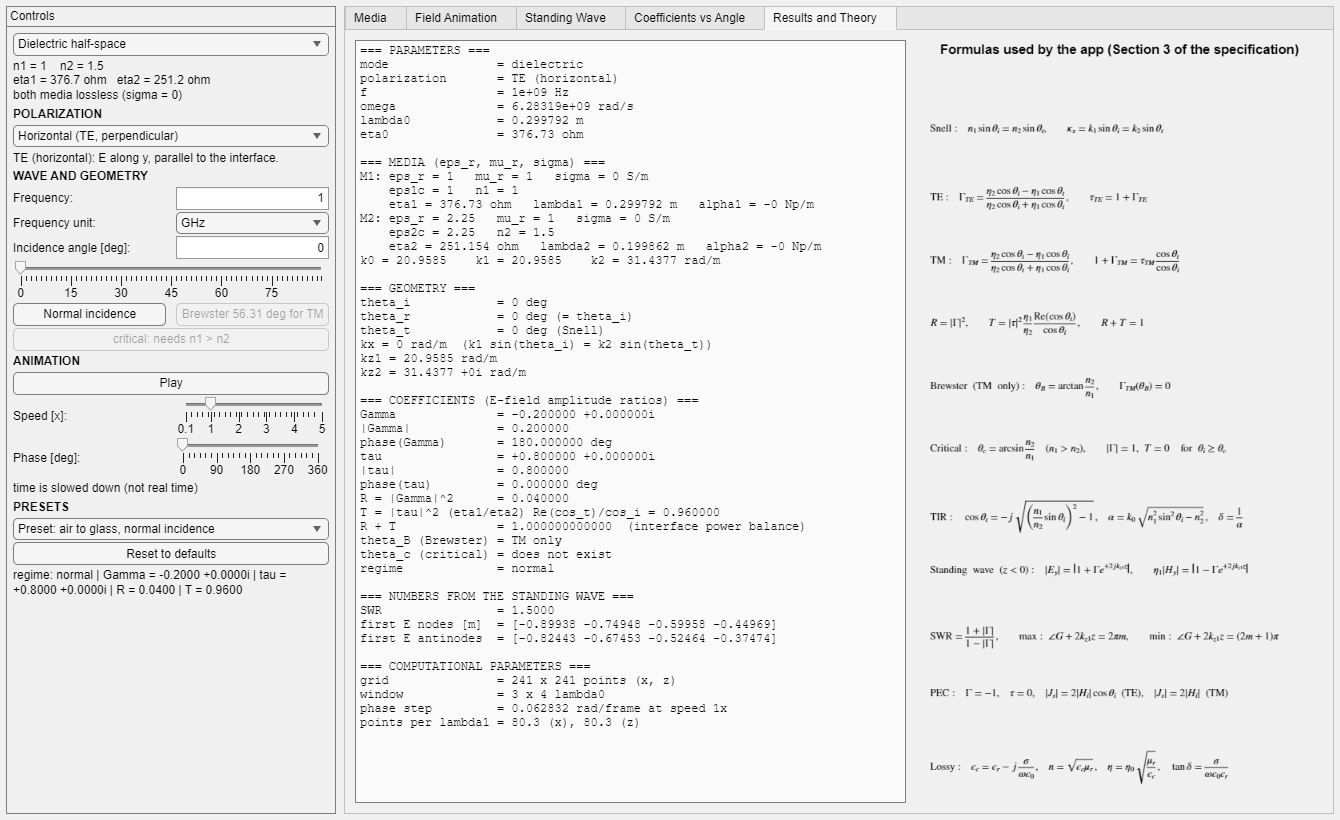
\includegraphics[width=0.98\textwidth]{fig6_gui_results.png}
  \caption{تب \lr{Results and Theory:} پنل اعداد و پنل فرمول‌ها.}
\end{figure}
\begin{figure}[H]
  \centering
  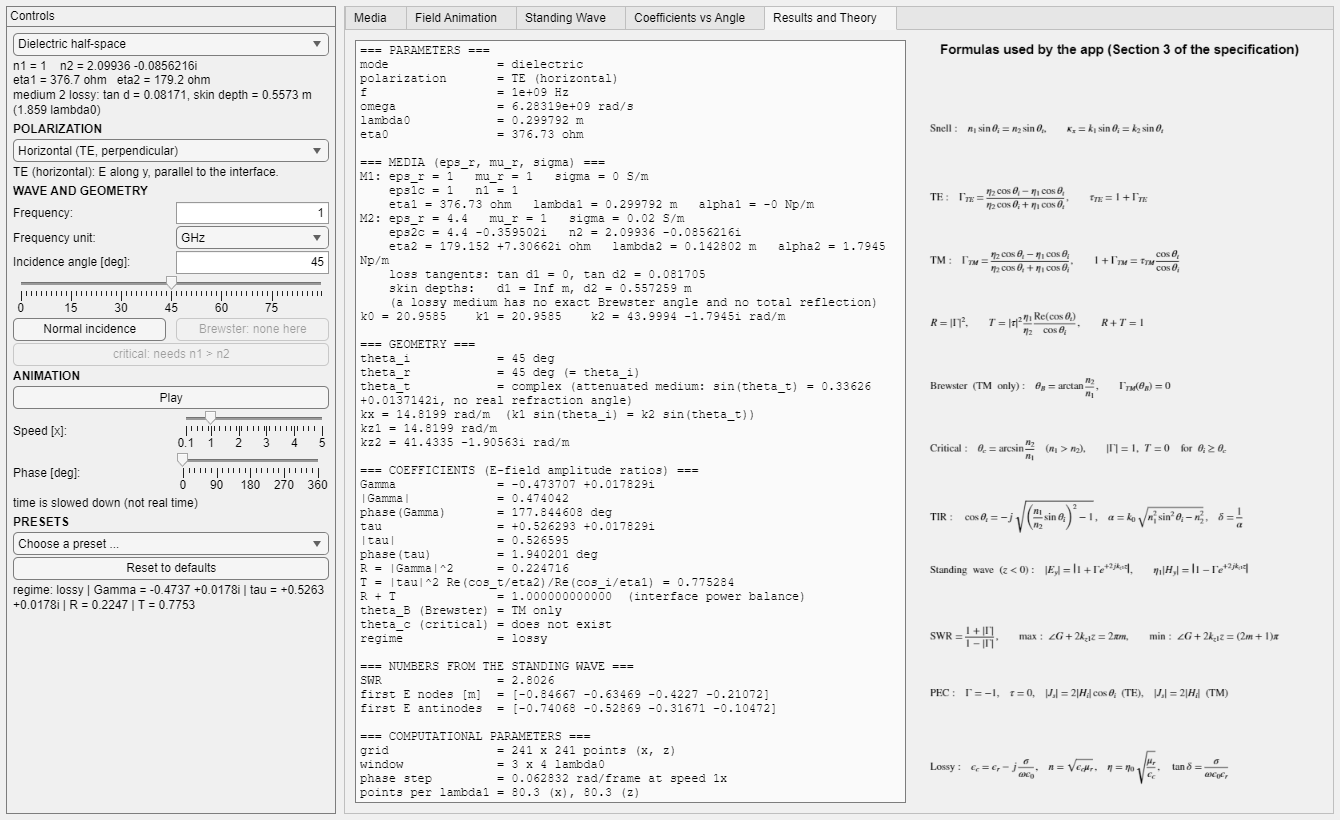
\includegraphics[width=0.98\textwidth]{guide_results_lossy.png}
  \caption{همان تب برای محیط اتلافی: بلوک‌های گذردهی مختلط، ثابت تضعیف، تانژانت اتلاف و عمق پوست به اعداد اضافه می‌شوند.}
\end{figure}

\section{جدول کامل کنترل‌ها}
\begin{table}[H]
  \centering
  \small
  \caption{کنترل‌های برنامه}
  \begin{tabular}{|p{5.0cm}|p{3.6cm}|p{7.8cm}|}
    \hline
    \textbf{کنترل} & \textbf{محل} & \textbf{کار} \\
    \hline
    \lr{Simulation mode} & پنل چپ & انتخاب محیط ۲: دی‌الکتریک یا رسانای کامل \\
    \hline
    خلاصۀ محیط‌ها & پنل چپ & نمایش $n_1$ و $n_2$ و $\eta_1$ و $\eta_2$ و وضعیت اتلاف یا مغناطیسی \\
    \hline
    \lr{Polarization} & پنل چپ & انتخاب قطبش افقی (\lr{TE)} یا عمودی (\lr{TM)} \\
    \hline
    \lr{Frequency} & پنل چپ & بسامد با واحد مگاهرتز یا گیگاهرتز \\
    \hline
    \lr{Incidence angle} & پنل چپ & زاویۀ فرود با کادر عددی و لغزنده \\
    \hline
    \lr{Normal incidence} & پنل چپ & تنظیم زاویه روی صفر درجه \\
    \hline
    \lr{Brewster} / \lr{critical} & پنل چپ & پرش به زاویۀ بروستر یا بحرانی، اگر وجود داشته باشد \\
    \hline
    \lr{Play} / \lr{Pause} & پنل چپ & شروع و توقف انیمیشن \\
    \hline
    \lr{Speed} و \lr{Phase} & پنل چپ & سرعت انیمیشن و فاز لحظه‌ای \\
    \hline
    \lr{Presets} & پنل چپ & ده سناریوی آماده \\
    \hline
    \lr{Reset to defaults} & پنل چپ & بازگرداندن همۀ مقادیر به حالت اولیه \\
    \hline
    $\varepsilon_r$ و $\mu_r$ و \lr{\texttt{sigma}} & تب \lr{Media} & شش ثابت محیط ۱ و ۲ \\
    \hline
    \lr{Quick material} & تب \lr{Media} & پرکردن سریع محیط ۲ با مادۀ آماده \\
    \hline
    \lr{Swap media 1}$<$-$>$2 & تب \lr{Media} & جابه‌جایی دو محیط برای رسیدن به بازتاب کلی \\
    \hline
    \lr{Incident} و \lr{Reflected} و \lr{Transmitted} & نوار ابزار تب اول & انتخاب موج‌های نمایش‌داده‌شده \\
    \hline
    \lr{E map} و \lr{H map} & نوار ابزار تب اول & انتخاب مؤلفۀ رسم‌شده در هر نقشه \\
    \hline
    \lr{Window} & نوار ابزار تب اول & اندازۀ پنجرۀ نمایش برحسب طول موج \\
    \hline
    \lr{R} و \lr{T} یا اندازۀ ضرایب & تب ضرایب & تغییر کمیت رسم‌شده در چهار نمودار \\
    \hline
  \end{tabular}
\end{table}

چرا بعضی دکمه‌ها غیرفعال‌اند؟ برچسب خود دکمه دلیل را می‌گوید. زاویۀ بحرانی تنها با دو محیط بدون اتلاف و شرط $n_1$ $>$ $n_2$ وجود دارد؛ برای رسیدن به آن دکمۀ جابه‌جایی محیط‌ها را بزنید. زاویۀ بروستر در محیط بدون اتلاف و غیرمغناطیسی فقط برای قطبش \lr{TM} وجود دارد و در محیط مغناطیسی ممکن است به قطبش \lr{TE} منتقل شود. نگه‌داشتن نشانگر روی دکمه همین توضیح را نشان می‌دهد.

\section{روابط فیزیکی که برنامه حل می‌کند}
\begin{table}[H]
  \centering
  \small
  \caption{روابط اصلی}
  \begin{tabular}{|p{4.6cm}|p{11.8cm}|}
    \hline
    \textbf{کمیت} & \textbf{رابطه} \\
    \hline
    قانون اسنل & $n_1\sin\theta_i=n_2\sin\theta_t$ \\
    \hline
    پایستگی عدد موج مماسی & $k_x=k_1\sin\theta_i=k_2\sin\theta_t$ \\
    \hline
    قطبش \lr{TE} & $\Gamma=\frac{\eta_2\cos\theta_i-\eta_1\cos\theta_t}{\eta_2\cos\theta_i+\eta_1\cos\theta_t},\quad \tau=1+\Gamma$ \\
    \hline
    قطبش \lr{TM} & $\Gamma=\frac{\eta_2\cos\theta_t-\eta_1\cos\theta_i}{\eta_2\cos\theta_t+\eta_1\cos\theta_i},\quad 1+\Gamma=\tau\frac{\cos\theta_t}{\cos\theta_i}$ \\
    \hline
    توان & $R=|\Gamma|^2,\quad T=|\tau|^2\frac{\eta_1}{\eta_2}\frac{\mathrm{Re}(\cos\theta_t)}{\cos\theta_i},\quad R+T=1$ \\
    \hline
    زاویۀ بروستر & $\theta_B=\arctan(n_2/n_1)$ برای \lr{TM} در محیط بدون اتلاف و غیرمغناطیسی \\
    \hline
    زاویۀ بحرانی & $\theta_c=\arcsin(n_2/n_1)$ با شرط $n_1$ $>$ $n_2$ \\
    \hline
    بازتاب کلی & $\cos\theta_t=-j\sqrt{(n_1\sin\theta_i/n_2)^2-1}$ \\
    \hline
    پوش موج ایستا & $|E_y|=|1+\Gamma e^{2jk_{z1}z}|$ \\
    \hline
    نسبت موج ایستا & $\mathrm{SWR}=\frac{1+|\Gamma|}{1-|\Gamma|}$ \\
    \hline
    رسانای کامل & $\Gamma=-1,\ \tau=0,\ |J_s|=2|H_i|\cos\theta_i\ (\mathrm{TE}),\ 2|H_i|\ (\mathrm{TM})$ \\
    \hline
  \end{tabular}
\end{table}

\section{اعتبارسنجی: مقایسۀ تحلیلی و عددی}

هر ردیف جدول زیر دو بار محاسبه شده است: یک بار از فرمول تحلیلی و یک بار از هستۀ محاسباتی برنامه. ستون آخر را با محاسبۀ دستی خودتان پر کنید. جدول کامل با ۳۷ ردیف در فایل \lr{docs/}\lr{\texttt{VALIDATION.md}} موجود است.
\begin{longtable}{|p{0.8cm}|p{6.4cm}|p{3.4cm}|p{3.4cm}|p{2.4cm}|}
  \caption{مقایسه مقادیر تحلیلی و محاسبه‌شده (ستون آخر برای محاسبه دستی)}\label{tab:val}\\
  \hline
  \textbf{\lr{\#}} & \textbf{کمیت} & \textbf{تحلیلی} & \textbf{محاسبه برنامه} & \textbf{دستی} \\
  \hline
  \endfirsthead
  \hline
  \textbf{\lr{\#}} & \textbf{کمیت} & \textbf{تحلیلی} & \textbf{محاسبه برنامه} & \textbf{دستی} \\
  \hline
  \endhead
  1 & \lr{air-}$>$\lr{glass normal: Gamma} & -0.2 & -0.2 &  \\
  \hline
  2 & \lr{air-}$>$\lr{glass normal: tau} & 0.8 & 0.8 &  \\
  \hline
  3 & \lr{air-}$>$\lr{glass normal: R} & 0.04 & 0.04 &  \\
  \hline
  4 & \lr{air-}$>$\lr{glass normal: T} & 0.96 & 0.96 &  \\
  \hline
  5 & \lr{air-}$>$\lr{glass normal: SWR} & 1.5 & 1.5 &  \\
  \hline
  6 & \lr{air-}$>$\lr{glass 45 deg: Gamma\_TE} & -0.3033370453 & -0.3033370453 &  \\
  \hline
  7 & \lr{air-}$>$\lr{glass 45 deg: Gamma\_TM} (\lr{spec sign)} & -0.09201336305 & -0.09201336305 &  \\
  \hline
  8 & \lr{air-}$>$\lr{glass 45 deg: Gamma\_TM} (\lr{other books,} -\lr{x)} & 0.09201336305 & 0.09201336305 &  \\
  \hline
  9 & \lr{air-}$>$\lr{glass 45 deg: theta\_t} [\lr{deg]} & 28.1255057 & 28.1255057 &  \\
  \hline
  10 & \lr{air-}$>$\lr{glass: theta\_B} [\lr{deg]} & 56.30993247 & 56.30993247 &  \\
  \hline
  11 & \lr{air-}$>$\lr{glass:} & \lr{Gamma\_TM(theta\_B)} &  &  \\
  \hline
  12 & \lr{air-}$>$\lr{glass: theta\_t(theta\_B)} [\lr{deg]} & 33.69006753 & 33.69006753 &  \\
  \hline
  13 & \lr{glass-}$>$\lr{air: theta\_c} [\lr{deg]} & 41.8103149 & 41.8103149 &  \\
  \hline
  14 & \lr{glass-}$>$\lr{air 60 deg: alpha} [1/\lr{m]} & 17.37782889 & 17.37782889 &  \\
  \hline
  15 & \lr{glass-}$>$\lr{air 60 deg: delta} [\lr{m]} & 0.05754458778 & 0.05754458778 &  \\
  \hline
  16 & \lr{glass-}$>$\lr{air 60 deg:} & \lr{Gamma\_TE} &  &  \\
  \hline
  17 & \lr{glass-}$>$\lr{air 60 deg: T} & 0 & 0 &  \\
  \hline
  18 & \lr{PEC normal: Gamma} & -1 & -1 &  \\
  \hline
  19 & \lr{PEC normal:} & \lr{Js} & [\lr{A/m]} &  \\
  \hline
  20 & \lr{PEC normal:} & \lr{Ey} & \lr{at z} = -0.31 \lr{lambda1} &  \\
  \hline
  21 & \lr{TM 50 deg: max} & \lr{tangential E jump} &  &  \\
  \hline
  22 & \lr{TM 50 deg: max} & \lr{tangential H jump} &  &  \\
  \hline
  23 & \lr{TM 50 deg: max} & \lr{eps Ez jump} &  &  \\
  \hline
  24 & \lr{TM 50 deg: R} + \lr{T} - 1 & 0 & 0 &  \\
  \hline
  25 & \lr{TM 50 deg: Sz(medium 1)} - \lr{Sz(medium 2)} & 0 & -4.33680869\lr{e-19} &  \\
  \hline
  26 & \lr{lossy FR-4: Re(}$\varepsilon_c$) & 4.4 & 4.4 &  \\
  \hline
  27 & \lr{lossy FR-4:} -\lr{Im(}$\varepsilon_c$) & 0.3595020715 & 0.3595020715 &  \\
  \hline
  28 & \lr{lossy FR-4: loss tangent} & 0.08170501625 & 0.08170501625 &  \\
  \hline
  29 & \lr{lossy FR-4: alpha} [\lr{Np/m]} & 1.794496971 & 1.794496971 &  \\
  \hline
  30 & \lr{lossy FR-4: skin depth} [\lr{m]} & 0.5572592298 & 0.5572592298 &  \\
  \hline
  31 & \lr{lossy FR-4: R} + \lr{T} - 1 (\lr{interface balance)} & 0 & 0 &  \\
  \hline
  32 & \lr{lossy FR-4 TM 35 deg: R} + \lr{T} - 1 & 0 & 0 &  \\
  \hline
  33 & \lr{magnetic:} $n_2$ = \lr{sqrt(}$\varepsilon_r$ $\mu_r$) & 3 & 3 &  \\
  \hline
  34 & \lr{magnetic: eta2} = \lr{eta0 sqrt(}$\mu_r$/$\varepsilon_r$) & 502.3070846 & 502.3070846 &  \\
  \hline
  35 & \lr{magnetic: Gamma at normal incidence} & 0.1428571429 & 0.1428571429 &  \\
  \hline
  36 & \lr{magnetic: TE Brewster angle} [\lr{deg]} & 43.08872314 & 43.08872411 &  \\
  \hline
  37 & \lr{TIR:} & \lr{E(z+delta)} & / &  \\
  \hline
\end{longtable}

آنچه با اجرای واقعی تأیید شده است: آزمون‌های \lr{\texttt{test\_core}} یعنی \lr{T1} تا \lr{T12} همه \lr{PASS} شده‌اند؛ از جمله شرط‌های مرزی روی آرایه‌های میدان با خطای کمتر از $6\times10^{-16}$، برابری $R+T=1$، پیوستگی مؤلفۀ \lr{z} بردار پوینتینگ، میدان میرای بازتاب کلی، محیط اتلافی و محیط مغناطیسی. آزمون خودکار رابط گرافیکی ۴۹ بررسی را بدون خطا گذرانده و پویش ۱۰۶ حالتی هیچ خطای عددی پیدا نکرده است. اجرای رابط به‌صورت خودکار و بدون نمایش انجام شده؛ لطفاً یک‌بار خودتان برنامه را باز کنید و ظاهر و انیمیشن را ببینید.

\section{عیب‌یابی و پرسش‌های متداول}
\begin{table}[H]
  \centering
  \small
  \caption{مشکل‌ها و راه‌حل‌ها}
  \begin{tabular}{|p{5.6cm}|p{10.8cm}|}
    \hline
    \textbf{مشکل} & \textbf{راه‌حل} \\
    \hline
    پنجره بسته نمی‌شود یا پس از تغییر فایل‌ها خطا می‌دهد & متلب نسخۀ قدیمی فایل را در حافظه دارد؛ در پنجرۀ فرمان \lr{delete(findall(groot,'Type','figure'))} را اجرا کنید و سپس \lr{\texttt{run\_lab}}. \\
    \hline
    دکمۀ زاویۀ بحرانی غیرفعال است & زاویۀ بحرانی فقط با $n_1$ $>$ $n_2$ و دو محیط بدون اتلاف وجود دارد. در تب \lr{Media} دکمۀ \lr{Swap media} را بزنید یا از پیش‌تنظیم بازتاب کلی استفاده کنید. \\
    \hline
    دکمۀ بروستر غیرفعال است & در محیط غیرمغناطیسی زاویۀ بروستر فقط برای \lr{TM} است؛ برچسب دکمه می‌گوید زاویه برای کدام قطبش وجود دارد. در محیط مغناطیسی ممکن است برعکس شود. \\
    \hline
    در تب موج ایستا \lr{SWR} تعریف‌نشده است & محیط ۱ اتلافی است؛ برای دیدن \lr{SWR} مقدار \lr{\texttt{sigma1}} را صفر کنید. \\
    \hline
    زاویۀ ۹۰ درجه پذیرفته نمی‌شود & در فرود مماسی \lr{cos} $\theta_i$ صفر می‌شود و روابط \lr{T} و فاصلۀ گره‌ها تکین می‌شوند؛ بیشینه ۸۹.۹ درجه است. \\
    \hline
    گره‌ای در تب موج ایستا نمی‌بینم & اگر دو محیط یکسان باشند $\Gamma=0$ است و موج بازتابی وجود ندارد؛ همچنین فرم بستۀ گره‌ها فقط برای محیط ۱ بدون اتلاف معتبر است. \\
    \hline
    انیمیشن کند یا سریع است & سرعت با لغزندۀ \lr{Speed} تنظیم می‌شود و مستقل از بسامد واقعی است؛ زمان نمایش عمداً کند شده است. \\
    \hline
    $\varepsilon_r$ کوچک‌تر از یک وارد کردم & برنامه می‌پذیرد ولی \lr{n} $<$ 1 یعنی سرعت فاز بیش از سرعت نور و چنین دی‌الکتریک غیرفعالی وجود ندارد؛ فقط برای مطالعۀ پارامتری است. \\
    \hline
  \end{tabular}
\end{table}

\section{محدودیت‌های مدل}
\begin{itemize}[rightmargin=1.2em,itemsep=2pt,topsep=3pt,label={$\bullet$}]
  \item محیط‌ها همسان‌گرد و غیرمغناطیسی یا مغناطیسی با $\mu_r$ حقیقی هستند؛ اتلاف مغناطیسی مدل نشده است.
  \item محیط اتلافی زاویۀ بروستر دقیق و بازتاب کلی واقعی ندارد و برنامه «\lr{none}» گزارش می‌کند.
  \item اگر محیط ۱ اتلافی باشد \lr{SWR} تعریف‌نشده است و مکان گره‌ها فقط به‌صورت عددی یافت می‌شود.
  \item برخورد مایل دوبعدی است؛ نمای سه‌بعدی پرتو و بردار پوینتینگ پیاده‌سازی نشده است.
  \item فاز انیمیشن گامی ثابت در هر فریم دارد و متناسب با زمان واقعی نیست.
  \item در حالت $|\Gamma|=1$ مقدار \lr{SWR} بی‌نهایت گزارش می‌شود.
\end{itemize}

\section{پیوست: پرسش‌های ارائۀ شفاهی}

پاسخ کوتاه این پرسش‌ها در فایل \lr{docs/}\lr{\texttt{THEORY\_MAP.md}} آمده است.
\begin{itemize}[rightmargin=1.2em,itemsep=2pt,topsep=3pt,label={$\bullet$}]
  \item چرا برای قطبش \lr{TE} زاویۀ بروستر وجود ندارد؟
  \item چرا علامت $\Gamma$ در قطبش \lr{TM} در زاویۀ بروستر تغییر می‌کند؟
  \item در بازتاب کلی فاز $\Gamma$ چقدر است و آیا توانی عبور می‌کند؟
  \item چرا موج میرا با پایستگی انرژی تناقض ندارد؟
  \item چرا باید شاخۀ $\mathrm{Im}(\cos\theta_t)<0$ انتخاب شود؟
  \item چرا برای رسانای کامل $\Gamma=-1$ و $\tau=0$ است و جریان سطحی از کجا می‌آید؟
  \item چرا عدد موج مماسی در مرز پایسته است؟
  \item گره‌های میدان برای \lr{TE} و \lr{TM} روی رسانای کامل کجا هستند؟
  \item چرا در رابطۀ \lr{T} ضریب $\frac{\eta_1}{\eta_2}\frac{\cos\theta_t}{\cos\theta_i}$ ظاهر می‌شود؟
  \item فاز انیمیشن چه نسبتی با زمان واقعی دارد؟
  \item چرا محیط اتلافی بازتاب کلی و زاویۀ بروستر دقیق ندارد؟
  \item چرا در محیط اتلافی همچنان $R+T=1$ است؟
  \item چرا در محیط مغناطیسی زاویۀ بروستر به قطبش \lr{TE} منتقل می‌شود؟
\end{itemize}

\end{document}
